\documentclass[10.5pt]{article}
\usepackage{amsmath,amssymb,amsthm}
\usepackage{listings}
\usepackage{graphicx}
\usepackage[shortlabels]{enumitem}
\usepackage{tikz}
\usepackage[margin=1in]{geometry}
\usepackage{fancyhdr}
\usepackage{epsfig} %% for loading postscript figures
\usepackage{amsmath}
\usepackage{float}
\usepackage{amssymb}
\usepackage{caption}
\usepackage{subfigure}
\usepackage{graphics}
\usepackage{titlesec}
\usepackage{mathrsfs}
\usepackage{amsfonts}
\usepackage{indentfirst}
\usepackage{fancybox}
\usepackage{tikz}
\usepackage{algorithm}
\usepackage{algorithmic}
\usepackage{array}

\renewcommand{\baselinestretch}{1.2}%Adjust Line Spacing
%\geometry{left=2.0cm,right=2.0cm,top=2.0cm,bottom=2.0cm}% Adjust Margins of the File
\usepackage{tikz-qtree}
\usetikzlibrary{graphs}
\tikzset{every tree node/.style={minimum width=2em,draw,circle},
	blank/.style={draw=none},
	edge from parent/.style=
	{draw,edge from parent path={(\tikzparentnode) -- (\tikzchildnode)}},
	level distance=1.2cm}
\setlength{\parindent}{0pt}
%\setlength{\parskip}{5pt plus 1pt}
\setlength{\headheight}{13.6pt}
\newcommand\question[2]{\vspace{.25in}\hrule\textbf{#1: #2}\vspace{.5em}\hrule\vspace{.10in}}
\renewcommand\part[1]{\vspace{.10in}\textbf{(#1)}}
%\newcommand\algorithm{\vspace{.10in}\textbf{Algorithm: }}
\newcommand\correctness{\vspace{.10in}\textbf{Correctness: }}
\newcommand\runtime{\vspace{.10in}\textbf{Running time: }}
\pagestyle{fancyplain}
% Create horizontal rule command with an argument of height
\newcommand{\horrule}[1]{\rule{\linewidth}{#1}}
% Set the title here
\title{
	\normalfont \normalsize
	\textsc{ShanghaiTech University} \\ [25pt]
	\horrule{0.5pt} \\[0.4cm] % Thin top horizontal rule
	\huge CS101 Algorithms and Data Structures\\ % The assignment title
	\LARGE Fall 2021\\
	\LARGE Homework 9\\
	\horrule{2pt} \\[0.5cm] % Thick bottom horizontal rule
}
% wrong usage of \author, never mind
\author{}
\date{Due date: 23:59, December 5, 2021}

% set the header and footer
\pagestyle{fancy}
\lhead{CS101 Algorithms and Data Structures}
\chead{Homework 9}
\rhead{Due date: 23:59, December 5, 2021}
\cfoot{\thepage}
\renewcommand{\headrulewidth}{0.4pt}
\newtheorem{Q}{Question}
% special settings for the first page
\fancypagestyle{firstpage}
{
	\renewcommand{\headrulewidth}{0pt}
	\fancyhf{}
	\fancyfoot[C]{\thepage}
}

% Add the support for auto numbering
% use \problem{title} or \problem[number]{title} to add a new problem
% also \subproblem is supported, just use it like \subsection
\newcounter{ProblemCounter}
\newcounter{oldvalue}
\newcommand{\problem}[2][-1]{
	\setcounter{oldvalue}{\value{secnumdepth}}
	\setcounter{secnumdepth}{0}
	\ifnum#1>-1
	\setcounter{ProblemCounter}{0}
	\else
	\stepcounter{ProblemCounter}
	\fi
	\section{Problem \arabic{ProblemCounter}: #2}
	\setcounter{secnumdepth}{\value{oldvalue}}
}
\newcommand{\subproblem}[1]{
	\setcounter{oldvalue}{\value{section}}
	\setcounter{section}{\value{ProblemCounter}}
	\subsection{#1}
	\setcounter{section}{\value{oldvalue}}
}

\begin{document}
	\maketitle
	\thispagestyle{firstpage}
	%\newpage
	\vspace{3ex}
	
	\begin{enumerate}
		\item Please write your solutions in English. 
		
		\item Submit your solutions to gradescope.com.  
		
		\item Set your FULL Name to your Chinese name and your STUDENT ID correctly in Account Settings. 
		
		\item If you want to submit a handwritten version, scan it clearly. Camscanner is recommended. 
		
		\item When submitting, match your solutions to the according problem numbers correctly. 
		
		\item No late submission will be accepted.
		
		\item Violations to any of above may result in zero score. 
	\end{enumerate}
	
	\newpage
	
	%---------------------------------------------------------


\question{1}{(2'+2'+2') Multiple Choices}
	Each question has \textbf{one or more} correct answer(s). Please answer the following questions \textbf{according to  the definition specified in the lecture slides}.\\

	\textit{Note: Write down your answers in the table below. }
	\begin{table}[htbp]
		\begin{tabular}{|p{2cm}|p{2cm}|p{2cm}|p{2cm}|p{2cm}|p{2cm}|}
			\hline 
			Question 1 & Question 2 & Question 3 \\
			\hline 
			& &  \\ 
			\hline 
		\end{tabular} 
	\end{table}

	\begin{Q}
		Which of the following statements about \textbf{topological sort} is/are true?
		\begin{enumerate}[(A)]
			\item Any sub-graph of a DAG has a topological sorting.
			\item Any directed tree has a topological sorting.
			\item Implementation of topological sort requires $O(|V|)$ extra space.
			\item Since we have to scan all vertices to find those with zero in-degree in each iteration, the run time of topological sort is $\Omega(|V|^2)$.
		\end{enumerate}
	\end{Q}
	\vspace{0.5cm}

	\begin{Q}
		Which of the following statements about \textbf{Dijkstra’s algorithm} is/are true?
		\begin{enumerate}[(A)]
			\item Dijkstra’s algorithm can find the shortest path in any DAG.
			\item If we use Dijkstra’s algorithm, whether the graph is directed or undirected does not matter.
			\item If we implement Dijkstra’s algorithm with a binary min-heap, we may change keys of internal nodes in the heap.
			\item We prefer Dijkstra’s algorithm with binary heap implementation to the naive adjacency matrix implementation in a dense graph where $|E| = \Theta(|V|^2)$.
		\end{enumerate}
	\end{Q}
	\vspace{0.5cm}

	\begin{Q}
		Which of the following statements about \textbf{Bellman-Ford's algorithm} is/are true?
		\begin{enumerate}[(A)]
			\item Bellman-Ford's algorithm can find the shortest path for negative-weighted directed graphs without negative cycles while Dijkstra’s algorithm may fail.
			\item The run time of Bellman-Ford's algorithm is $O(|V||E|)$, which is more time-consuming than Dijkstra’s algorithm with heap implementation.
			\item Topological sort can be extended to determine whether a graph has a cycle while Bellman-Ford's algorithm can be extended to determine whether a graph has a negative cycle.
			\item Topological sort can find the critical path in a DAG while Bellman-Ford's algorithm can find the single-source shortest path in a DAG.
		\end{enumerate}
	\end{Q}
	\vspace{0.5cm}

\pagebreak

\question{2}{(5'+3') Topological Sort}


	Given the following DAG, run topological sort with a queue. Write down the vertex you select and update the in-degree \texttt{ind[i]} of all vertices in each iteration.  
	
	\textit{Note: When pushing several vertices into the queue at the same time, push them alphabetically. You are NOT required to show your queue at each step.}
	
	\vspace{1cm}

	\begin{figure}[htbp]
		\centering
		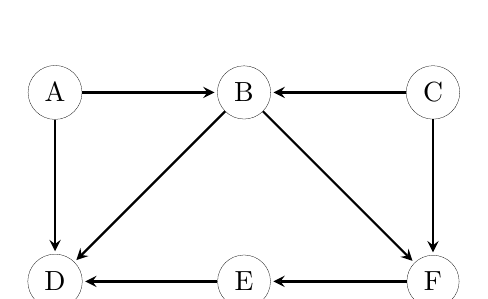
\begin{tikzpicture}[
			> = stealth, % arrow head style
			shorten > = 1pt, % don't touch arrow head to node
			node distance = 1cm, % distance between nodes
			thick, % line style
			scale = 0.8,
		]
		\node[circle, draw, line width=0.1pt] (a) at (-3,3){A};
		\node[circle, draw, line width=0.1pt] (b) at (0, 3){B};
		\node[circle, draw, line width=0.1pt] (c) at (3, 3){C};
		\node[circle, draw, line width=0.1pt] (d) at (-3,0){D};
		\node[circle, draw, line width=0.1pt] (e) at (0, 0){E};
		\node[circle, draw, line width=0.1pt] (f) at (3, 0){F};
		\draw[->] (a) to (b);
		\draw[->] (a) to (d);
		\draw[->] (b) to (d);
		\draw[->] (b) to (f);
		\draw[->] (c) to (b);
		\draw[->] (c) to (f);
		\draw[->] (f) to (e);
		\draw[->] (e) to (d);
		\end{tikzpicture}
	\end{figure}
	\vspace{0.5cm}

	\begin{table}[htbp]
		\begin{center}  
			\begin{tabular}{|l|c|l|l|l|l|l|l|}  
				\hline  
				 & vertex & \texttt{ind[A]} & \texttt{ind[B]} & \texttt{ind[C]} & \texttt{ind[D]} & \texttt{ind[E]} & \texttt{ind[F]}\\ \hline  
				initial     & / &   &   &   &   &   &   \\ \hline    
				iteration 1 &   &   &   &   &   &   &   \\ \hline    
				iteration 2 &   &   &   &   &   &   &   \\ \hline    
				iteration 3 &   &   &   &   &   &   &   \\ \hline    
				iteration 4 &   &   &   &   &   &   &   \\ \hline   
				iteration 5 &   &   &   &   &   &   &   \\ \hline    
				iteration 6 &   &   &   &   &   &   &   \\ 
				\hline  
			\end{tabular}  
		\end{center}
	\end{table}
	\vspace{0.5cm}

\begin{Q}
	Fill in the table above. What is the topological sorting that you obtain?
	\vspace{2cm}
\end{Q}

\begin{Q}
	How many different topological sortings does this graph have? Write them down.
\end{Q}

\pagebreak
%---------------------------------------------------------
\question{3}{(5'+3') Dijkstra's Algorithm}

	Given the following weighted graph, run Dijkstra's algorithm by considering $A$ as the source vertex. Write down the vertex you select and update current distance \texttt{dis[i]} of all vertices in each iteration.

	\vspace{1cm}

	\begin{figure}[htbp]
		\centering
		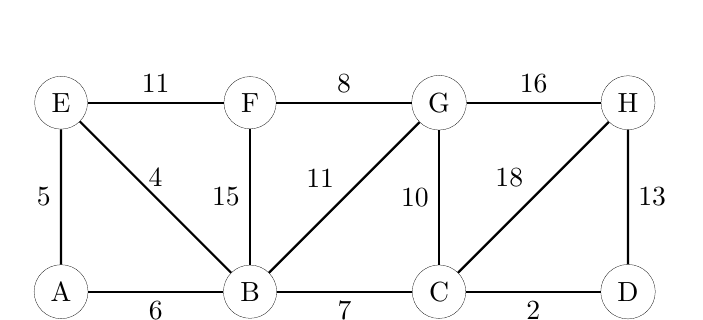
\begin{tikzpicture}
		[thick,scale=0.8, every node/.style={scale=1}]
		%		\node[circle] (n0){A};
		\node[circle, draw, line width=0.1pt] (a) at (-4.5,0){A};
		\node[circle, draw, line width=0.1pt] (b) at (-1.5,0){B};
		\node[circle, draw, line width=0.1pt] (c) at (1.5,0){C};
		\node[circle, draw, line width=0.1pt] (d) at (4.5,0){D};
		\node[circle, draw, line width=0.1pt] (e) at (-4.5,3){E};
		\node[circle, draw, line width=0.1pt] (f) at (-1.5,3){F};
		\node[circle, draw, line width=0.1pt] (g) at (1.5,3){G};
		\node[circle, draw, line width=0.1pt] (h) at (4.5,3){H};
		\draw[-] (a) to node[below]{6} (b);
		\draw[-] (a) to node[left]{5} (e);
		\draw[-] (b) to node[below]{7} (c);
		\draw[-] (b) to node[above]{4} (e);
		\draw[-] (b) to node[left]{15} (f);
		\draw[-] (b) to node[above left]{11} (g);
		\draw[-] (c) to node[below]{2} (d);
		\draw[-] (c) to node[left]{10} (g);
		\draw[-] (c) to node[above left]{18} (h);
		\draw[-] (d) to node[right]{13} (h);
		\draw[-] (e) to node[above]{11} (f);
		\draw[-] (f) to node[above]{8} (g);
		\draw[-] (g) to node[above]{16} (h);
		\end{tikzpicture}
	\end{figure}
	\vspace{0.5cm}

	

	\begin{Q}
		Fill in the table below.
		\begin{table}[htbp]
			\begin{center}  
				\begin{tabular}{|l|c|c|c|c|c|c|c|c|c| p{3cm}|}  
					\hline  
					& vertex & \texttt{dis[A]} & \texttt{dis[B]} & \texttt{dis[C]} & \texttt{dis[D]} & \texttt{dis[E]} & \texttt{dis[F]} & \texttt{dis[G]} & \texttt{dis[H]}\\ \hline  
					initial 	& / & 0 &$\infty$&$\infty$&$\infty$&$\infty$&$\infty$&$\infty$&$\infty$\\ \hline
					iteration 1 &   &   &   &   &   &   &   &   &  \\ \hline    
					iteration 2 &   &   &   &   &   &   &   &   &  \\ \hline    
					iteration 3 &   &   &   &   &   &   &   &   &  \\ \hline    
					iteration 4 &   &   &   &   &   &   &   &   &  \\ \hline    
					iteration 5 &   &   &   &   &   &   &   &   &  \\ \hline   
					iteration 6 &   &   &   &   &   &   &   &   &  \\ \hline    
					iteration 7 &   &   &   &   &   &   &   &   &  \\ \hline   
					iteration 8 &   &   &   &   &   &   &   &   &  \\  
					\hline  
				\end{tabular}  
			\end{center}  
		\end{table}
	\end{Q}

	\begin{Q}
		Fill in the table below for \textbf{time complexity analysis} of Dijkstra’s algorithm with different implementation. Write down your answer as simplified as possible.
		
		\textit{Hint: $\text{Total Run Time} = \texttt{pop()}\text{Time} \times |V| + \texttt{relax()}\text{Time} \times |E|$ for Dijkstra’s algorithm with adjacency list implementation, where \texttt{pop()} is the operation to find the unvisited vertex with least \texttt{dis[i]} in one iteration and \texttt{relax()} is the operation to update \texttt{dis[v]} according to \texttt{dis[u]} and weight of edge $(u, v)$. Heap implementation is based on adjacency list implementation.}
		\begin{table}[htbp]
			\begin{center}  
				\begin{tabular}{|l|p{3cm}<{\centering}|p{3cm}<{\centering}| p{3cm}<{\centering}|}  
					\hline  
					Implementation & \texttt{pop()} & \texttt{relax()}  & total \\ \hline  
					Adjacency Matrix&$O(|V|)$&$O(1)$& $O(|V|^2)$ \\ \hline
					Adjacency List 	&  		 &  	&  \\ \hline
					Binary Heap 	&  	     &  	& \\ \hline
					Fibonacci Heap 	&  		 &  	& \\ \hline
				\end{tabular}  
			\end{center}  
		\end{table}
	\end{Q}

\pagebreak

%---------------------------------------------------------	
\question{4}{(2'+3'+3')Providing Counterexamples}
For each of the following statements, provide counterexamples by \textbf{drawing a graph and briefly explaining it} to illustrate that these three statements are incorrect.
\begin{Q}
	Each DAG with $|V|$ vertices and $|V|-1$ edges has its unique topological sorting.
	\vspace{3.5cm}
\end{Q}

\begin{Q}
	Since we can find the \textbf{maximum spanning tree} in a graph by negating all edge weights by multiplying $-1$ and then running Prim's algorithm, similarly we can find the \textbf{longest path} in a positive-weighted graph by negating all weights and running Dijkstra's algorithm from every source node.
	\vspace{4cm}
\end{Q}
	
\begin{Q}
	Assume that we implement Dijkstra’s algorithm with a binary heap as the priority queue in a positive-weighted graph, then we can do the following operation: when the terminal vertex is pushed into the priority queue, we can stop the algorithm and return the correct shortest path from the source vertex to the terminal vertex, instead of keeping running the algorithm until popping the terminal vertex from the heap.
	\vspace{4cm}
\end{Q}

\end{document}